\chapter[2021 September]{September 2021}

\section[2021/09/03]{Sunday, 03 September 2021}

\subsection{STM32L072RZT6}

\subsubsection{Programming}

The STM32L0 series does not support \ac{JTAG} programming and rather only offers the \ac{SWD} programming interface. Therefore, the \ac{SWD} approach will be used to program the device. The \ac{SWD} programming interface requires the following 5 pins:

\begin{compactitem}
	\item SWDIO - Data input/output
	\item SWCLK - Clock signal
	\item NRST - Reset signal
	\item VDD - Supply voltage
	\item GND - Ground reference
\end{compactitem}

Note that the NRST pin is not actually necessary with \ac{SWD} interface programming since \ac{SWD} bypasses the bootloader and is capable of resetting and flashing the device directly.

\subsubsection{Power}

The STM32L072xx series supports a power supply of 1.65-3.6 V. However, this full range is only applicable under certain conditions. The microcontrollers in the series feature three power consumption ranges depending on the system's maximum operating frequency as well as the external voltage supply. Range 1 supports a CPU speed of up to the maximum 32 MHz but limits the $V_{DD}$ range to 1.71-3.6 V. Range 2 and 3 both support the full power supply range but only support a maximum CPU frequency of up to 16 MHz and 4.2 MHz respectively. For the purposes of this project, access to the full power supply range is not necessary. However, the use of the maximum CPU frequency of 32 MHz is preferable. Therefore, range 1 was selected as the power consumption range for the purposes of this project.

The $V_{DD}$ pins on the device can source a maximum of 100 mA individually and 105 mA combined while the $V_{SS}$ pins combined can sink a maximum of 100 mA individually and 105 mA combined. It needs to be ensured that the 3.3 V regulator powering the device is capable of supporting this current. Furthermore, all I/O pins except FTf pins can both sink and source a maximum output current of 16 mA individually. The total output current that can be sunk by all fo the I/O pins and control pins combined (excluding PA11 and PA12) is 90 mA. The total output current that can be sunk by I/O pins PA11 and PA12 is 25 mA. The total output current that can be sourced by all fo the I/O pins and control pins combined is 90 mA.

According to the general PCB design guidelines in the STM32L072x8/B/Z datasheet, $1\mu F$ ceramic decoupling capacitors in parallel with $100 nF$ ceramic decoupling capacitors should be connected across the power supply pins. $V_{DDA}$ indicates a pin dedicated to supply the ADC with power if a very clean and stable power source is required. For the purposes of this project, the ADC is only being used to monitor a pressure sensor. Therefore, high ADC performance is not required and it was decided to supply the ADC with the same power supply as for the rest of the device.

\subsubsection{General Notes}


\begin{compactitem}
	\item Unless otherwise specified by a note, all I/Os are set as floating inputs during and after reset.
	\item General PCB design guidelines are discussed on pg 105 of the datasheet.
\end{compactitem}

\subsection{Supporting Components}

The following components are required to support the operation of the STM32L072RZT6 microcontroller:

\begin{compactitem}
	\item 3.3 V regulator to step down 12 V input from the power supply to power the microcontroller. The TLV70233 from Texas Instruments is an example of a \ac{SMD} 3.3 V regulator that could potentially be used.
\end{compactitem}

\subsection{Pin Connections}

The pin connections for the STM32L072RZT6 are as follows:

\begin{compactitem}
	\item Pin 1 - $V_{DD}$
	\item Pin 5 - OSC\_IN
	\item Pin 6 - OSC\_OUT
	\item Pin 7 - NRST
	\item Pin 12 - $V_{SSA}$
	\item Pin 13 - $V_{DDA}$
	\item Pin 18 - $V_{SS}$
	\item Pin 19 - $V_{DD}$
	\item Pin 31 - $V_{SS}$
	\item Pin 32 - $V_{DD}$
	\item Pin 46 - SWDIO
	\item Pin 47 - $V_{SS}$
	\item Pin 48 - $V_{DD\_USB}$
	\item Pin 49 - SWCLK
	\item Pin 60 - BOOT0
	\item Pin 63 - $V_{SS}$
	\item Pin 64 - $V_{DD}$
\end{compactitem}

\pendsign

\section[2021/09/08]{Wednesday, 08 September 2021}

\subsection{Robotic Subsystem}

The mechanical assembly of the robotic subsystem was completed using chipboard wood as a base for the system. Furthermore, rubber feet were added to the base to reduce the effect of environmental vibrations on the system. The assembly is shown in \FigRef{fig:final-robotic-system}.

\begin{figure}[H]
	\centering
	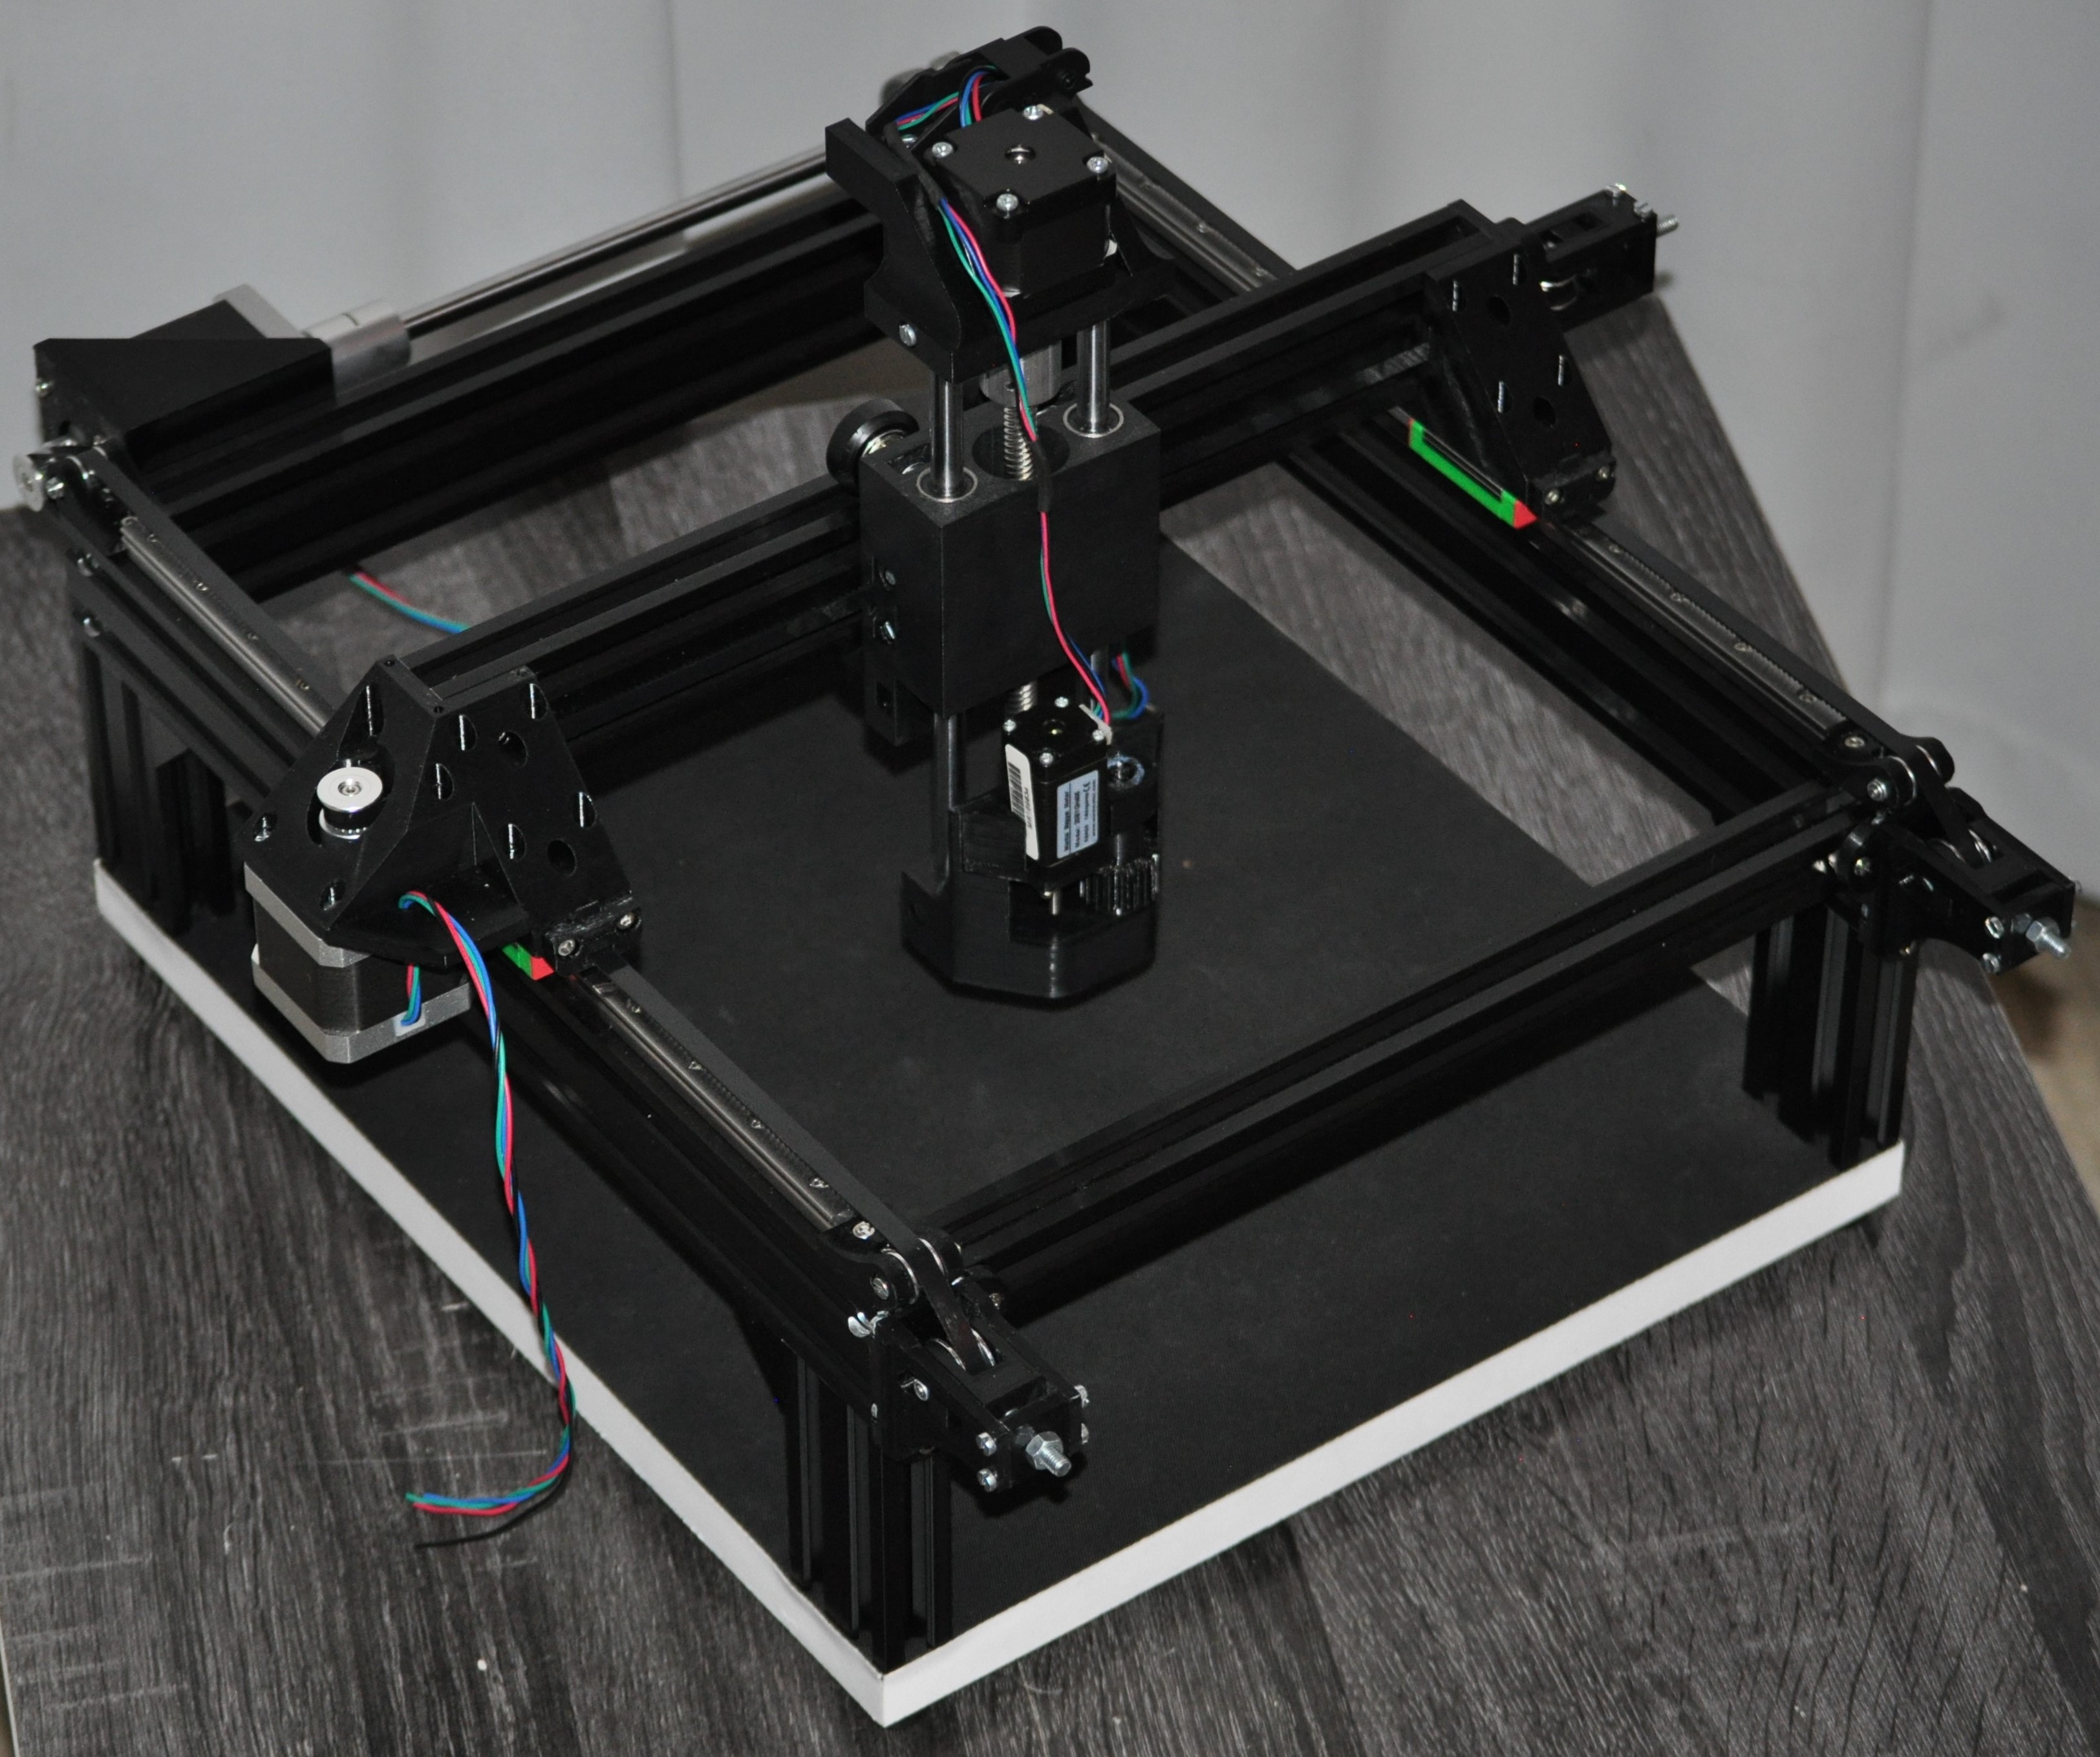
\includegraphics[width=0.7\linewidth]{figures/202109/final-robotic-system.JPG}
	\caption{Assembled mechanical component of robotic subsystem.}
	\label{fig:final-robotic-system}
\end{figure}

\subsection{External Oscillator}

The STM32L072RZT device supports the use of an external oscillator in the frequency range 1 to 24 MHz to drive the main clock. The advantage of using this oscillator over the main clock is the accuracy with which it operates in comparison to the internal oscillator.

\pendsign

\section[2021/09/11]{Saturday, 11 September 2021}

\subsection{PCB Design}

\subsubsection{Prototype}

The robotic controller prototype was created by soldering the STM32L072RZT6 microcontroller to a \ac{TQFP} breakout board with a pin pitch of 0.5mm. Due to the fine pitch of the pins, solder flux was required to be used in conjunction with the drag solder hand soldering technique for the process to be successful. Furthermore, several bridges formed during the initial drag solder pass which was removed using solder wick. Finally the solder flux residue was cleaned using \ac{IPA}. The final prototype is shown in \FigRef{fig:robotic-controller-prototype}.

\begin{figure}[H]
	\centering
	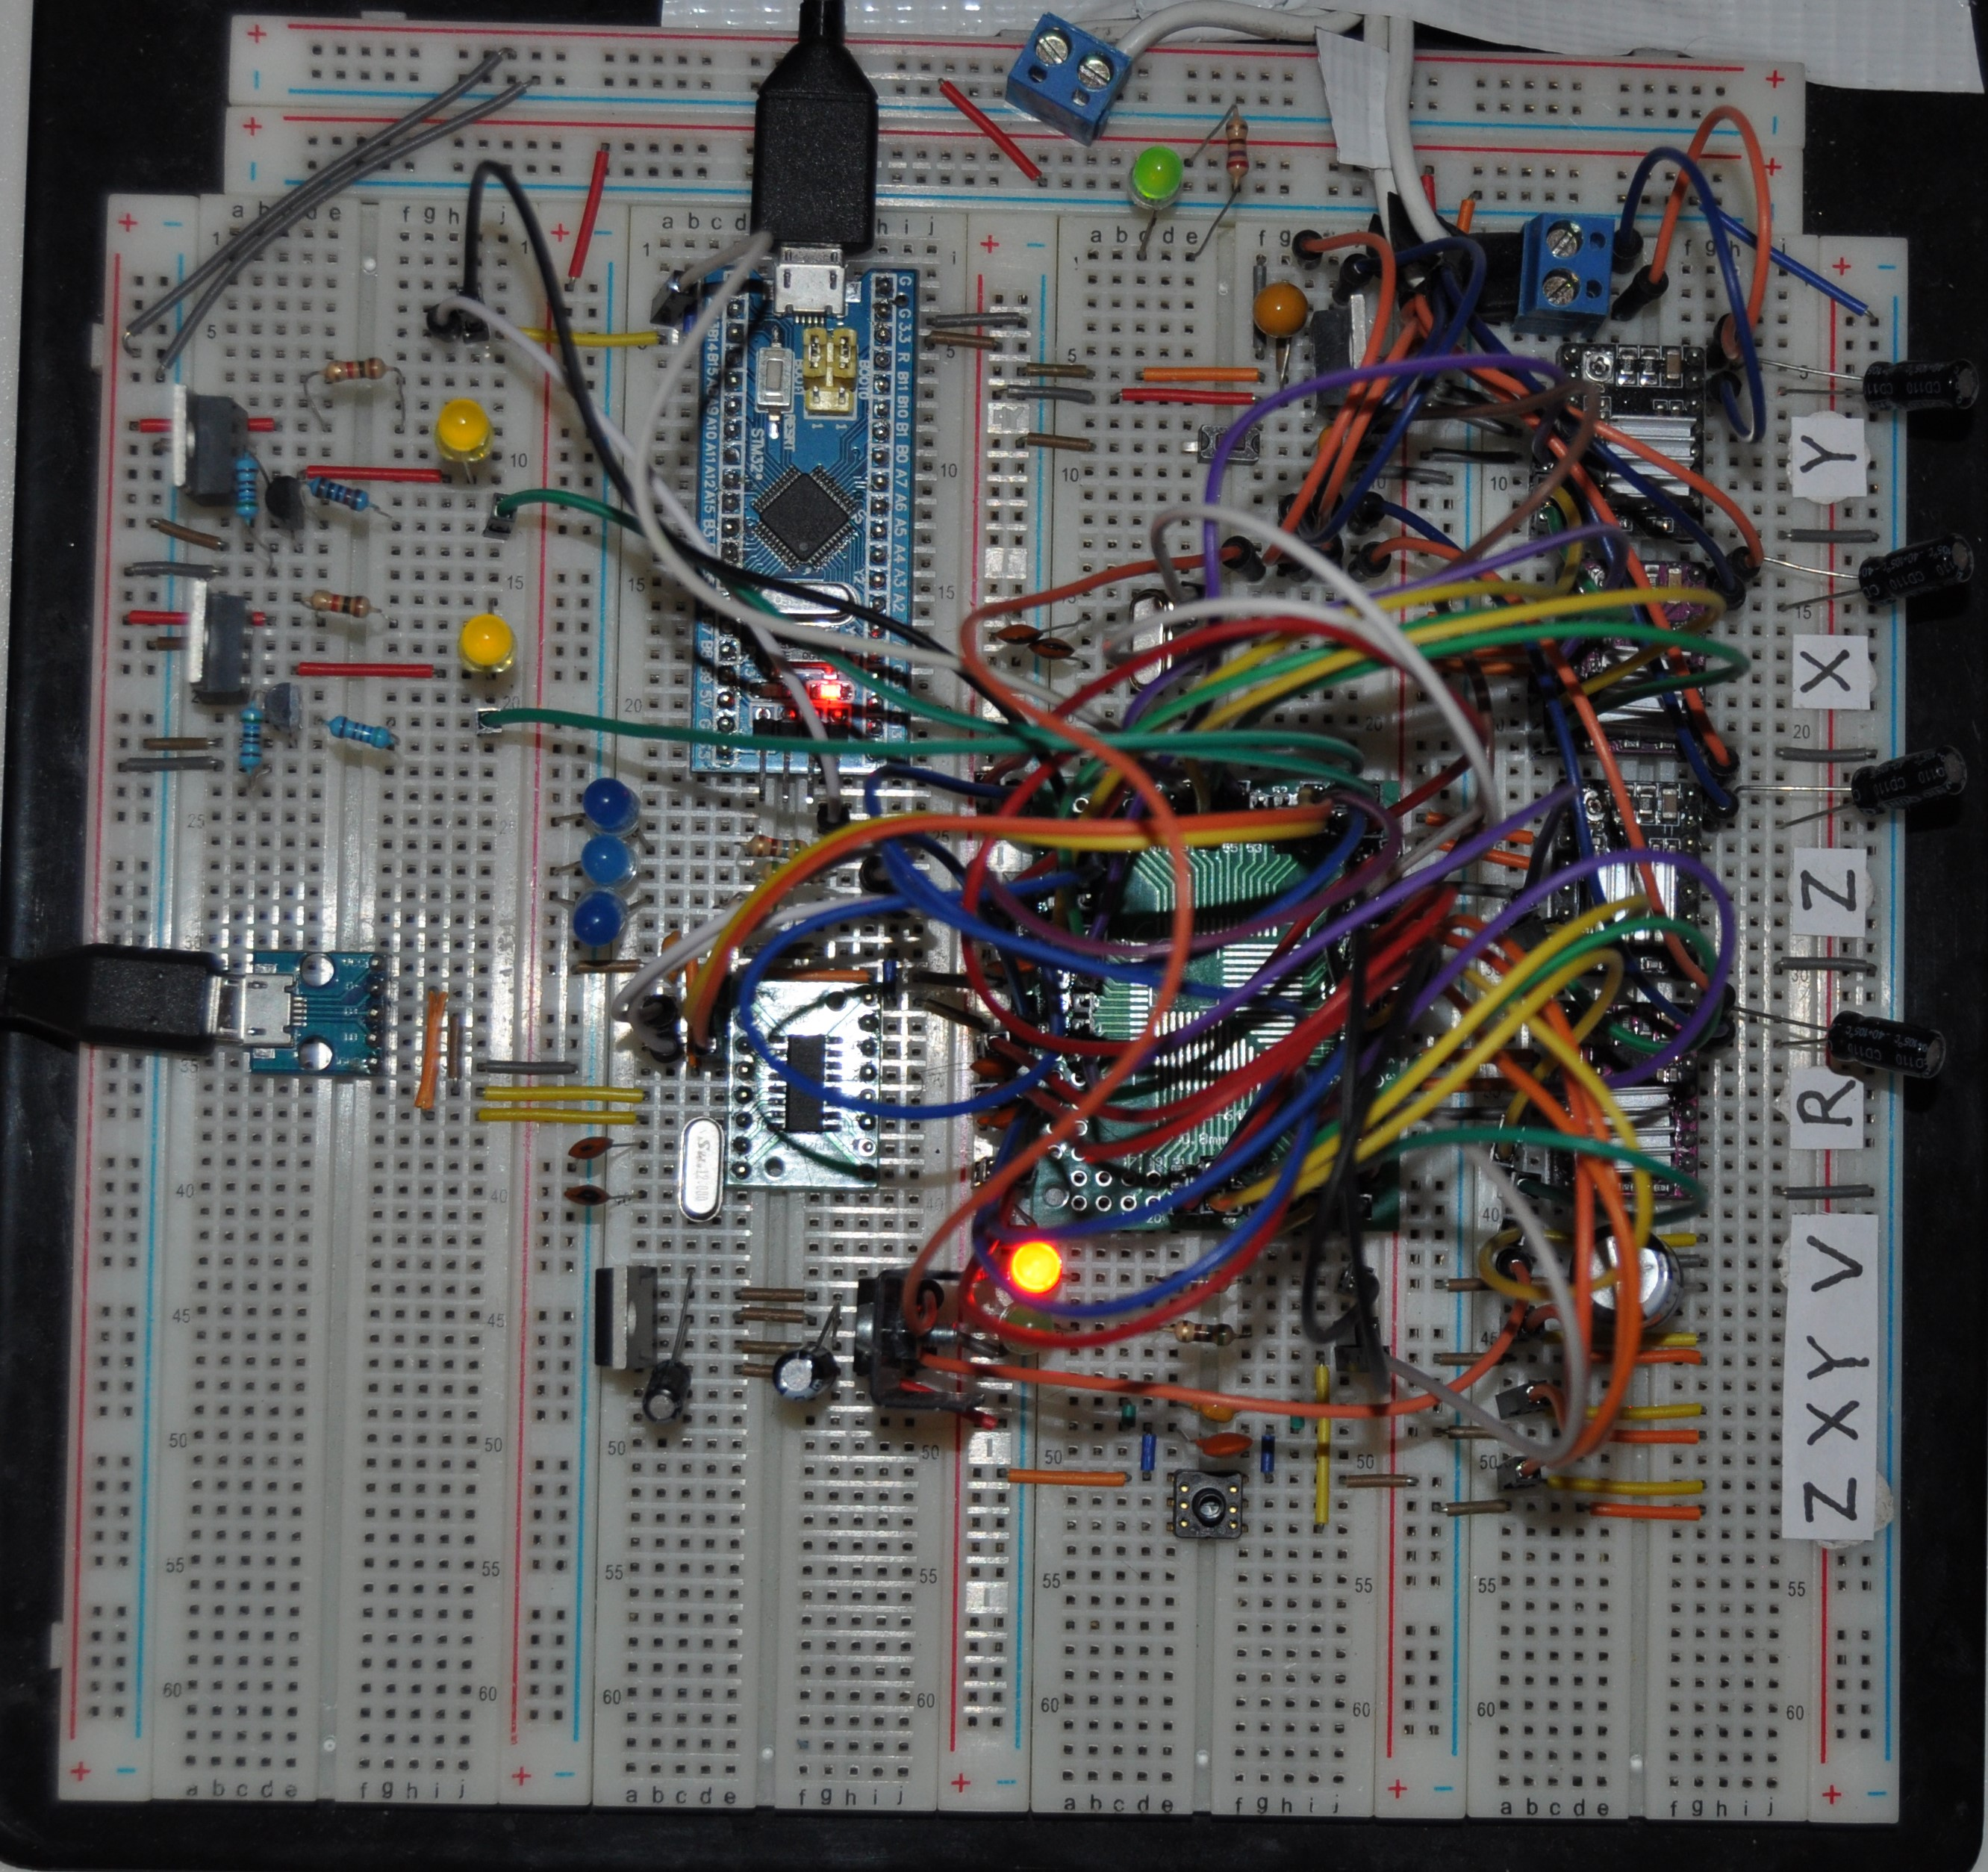
\includegraphics[width=0.7\linewidth]{figures/202109/robotic-controller-prototype.JPG}
	\caption{Robotic controller prototype.}
	\label{fig:robotic-controller-prototype}
\end{figure}


\subsubsection{Power}
The datasheet for the NCP1117 voltage regulators recommend the use of an input bypass capacitor if the device is significantly far away from the power source. The robotic controller PCB board is separate to the \ac{PSU} and connected by means of an arbitrary length of wire. Therefore, controller was designed with a $10\mu F$ ceramic 
capacitor across the input terminals of each NCP1117 voltage regulator. Similarly, in order to provide frequency compensation for the voltage regulator, the datasheet recommends a capacitor with a capacitance of at least $4.7\mu F$ is used. The capacitor may be of any type as long as it has an equivalent series resistance of between $33m\Omega$ and $2.2\Omega$. Therefore, it was decided to use the same capacitor as the bypass input capacitor which meets the stated requirements. Furthermore, this reduces the range of components required to be sourced.

In order to determine the width of the power supply trace, the maximum current that could flow on that trace needs to be known. Therefore, the maximum current draw of the components needs to be known. The maximum current ratings of each of the components are listed below.

\begin{compactitem}
	\item 42BYGHW920L21B2 - 2.2 A
	\item 42BYGHW609 stepper motor - 1.7 A
	\item 35BYGH312P1 stepper motor - 1.2 A
	\item 20BYGH406 stepper motor - 0.6 A
	\item DS3118MG servo motor - 2 A
	\item STM32L072RZT6 microcontroller - 105 mA
	\item CH340G chip - 30 mA
\end{compactitem}

Based on the sum of these values, the initial power connection trace needs to be able to support 5.835 A of current. A value of 6 A was used to incorporate a degree of engineering safety margin. Furthermore, a maximum temperature rise tolerance of $10\;^{\circ}C$ and a copper thickness of $1 \text{oz/ft}^2$ was used in the calculation of the trace width. Based on this, it was calculated a trace width of at least 140 mil or 3.56 mm is required. A similar procedure was used to calculate the power trace sections which supported fewer components. The board house, JLC PCB, charges a significantly greater amount for 2 oz outer copper weight over 1 oz. Therefore 1 oz was selected as the outer copper weight for the PCB. 

\subsection{USB Differential Routing}

The D+ and D- lines for the USB portion of the USB to serial converter constitute a differential pair. As such, a number of \ac{PCB} layout guidelines need to be adhered to ensure the integrity of the differential pair signal. The following guidelines were considered for this purpose:

\begin{compactitem}
	\item The use of vias should be minimised. In the case of the PCB for this project, vias were not used at all for the differential signal.
	\item The differential pair should be isolated from the other traces. This was achieved by enforcing a clearance of three standard trace widths from other traces for a total clearance of 0.75mm.
	\item Differential pair traces should mirror each other as far as possible.
	\item The lengths of each trace in the differential pair must be identical even if symmetry needs be sacrificed to achieve this.
\end{compactitem}

% https://resources.pcb.cadence.com/blog/2021-efficient-differential-pair-routing-guidelines-to-speed-up-pcb-routing


\subsection{Oscillator}

% See https://ecsxtal.com/crystal-and-oscillator-printed-circuit-board-design-considerations

\begin{compactitem}
	\item The crystal and its supporting capacitors should be placed as close as possible to the oscillator input and output pins on the microcontroller.
	\item The trace length in the oscillator circuit should be minimised.
	\item The traces in the oscillator circuit should not cross other signal lines.
	\item Traces should not incur right angle bends.
	\item The supporting capacitors should share a ground plane.
	\item The size of loops in the oscillator circuit should be minimised.
	\item The ground node should not pass under the crystal.
	\item Power and digital signal on other layers of the board should not pass under the crystal. 
\end{compactitem}

\subsection{LED Strip}

A white \ac{LED} strip was selected to provide sufficient lighting to support the computer vision component of the project. The \ac{LED} strip contains 3528 \ac{SMD} white LEDs which consume a maximum of 20 mA each. The \ac{LED} density of the strip is 60 LEDs/m. This project maximum LED strip length that this project will use is 3m which implies that a maximum of 180 LEDs will be powered. 

\pendsign

\section[2021/09/19]{Sunday, 19 September 2021}

\subsection{Vacuum Actuator}

The measured dimensions of the syringe tube are as follows:

\begin{compactitem}
	\item Outer diameter = 20.80 mm
	\item Inner diameter = 18.60 mm
	\item Length (excluding nozzle) = 97.00 mm
	\item Length (including nozzle) = 108.00 mm
	\item Nozzle length = 11.00 mm
	\item Nozzle base ridge diameter = 6.24 mm
	\item Nozzle base ridge height = 2.04 mm
	\item Nozzle base diameter = 4.50 mm
	\item Nozzle top outer diameter = 4.00 mm
	\item Nozzle top inner diameter = 2.14 mm
	\item Shortest distance from nozzle base to main outer tube outer diameter = 1.14 mm
	\item Flange diameter = 23.55 mm
	\item Flange overall length = 37.04 mm
	\item Flange thickness = 1.60 mm
	\item Flange edge length = 12.80 mm
\end{compactitem}

The dimensions of the syringe plunger are as follows:

\begin{compactitem}
	\item Flange diameter = 21.70 mm
	\item Flange thickness = 1.60 mm
	\item Flat strut width (wide section) = 18.00 mm
	\item Flat strut width (narrow section) = 13.24 mm
	\item Strut width transition offset from flange (initial) = 13.30 mm
	\item Strut width transition offset from flange (final) = 19.90 mm
	\item Length = 111.00 mm
	\item Rubber height = 9.609 mm 
	\item Flat strut thickness = 1.20 mm
	\item Rubber end piece height = 9.00 mm
\end{compactitem}

The syringe has a maximum range of linear travel of 78 mm. The servo has a maximum range of rotational motion of $180^{\circ}$. Therefore, in order to achieve the full range of linear motion for the syringe, the mechanism connecting the servo to the syringe needs to translate the servo's $180^{\circ}$ of rotational motion into 78 mm of linear motion. A rack and pinion system is a mechanism that is commonly used for converting translational motion into rotational motion. Therefore, half of the circumference of the pitch diameter circle of the gear needs to be equal to the length of linear travel for these specifications to be achieved. A gear with a pitch diameter of 49.66 mm satisfies this requirement. Therefore, it was selected to use a gear with a pitch diameter of 50 mm.

\pendsign

\section[2021/09/21]{Tuesday, 21 September 2021}

\subsection{Communication Protocol}

% See https://en.wikibooks.org/wiki/Serial_Programming/Forming_Data_Packets

A communication protocol needs to be developed between the robotic controller and the PC running the \ac{GUI} software. The PC needs to be able to issue the following commands to the robotic controller:

\begin{compactitem}
	\item Calibrate axes - The robot must home its motor to find the zero position on each axis as indicated when each limit switch is triggered. The robot must also place the rotational motor into sleep mode briefly to allow any rotational tension on the vacuum tube to be released. Following this the rotational motor must be removed from sleep mode and its current angular position reset as the zero angular position. 
	\item Go to position - The robot must move to the specified position in 3D Cartesian space as well as the specified z-axis angular position.
	\item Actuate vacuum mechanism - Set the actuation of the servo motor controlling the vacuum mechanism
	\item Report pressure in vacuum system
\end{compactitem}

\subsection{Firmware}

\subsubsection{Project Setup}

STM32CubeIDE was selected as the IDE of choice to develop the firmware for the microcontroller. The IDE was used to create an empty project that only contained essential board startup code and C library files. In order to use the STM32 register and peripheral aliases, the following files needed to be sourced from external sources and included under the includes folder in the project:

\begin{compactitem}
	\item stm32l0xx.h - This header file contains the \ac{CMSIS} definitions for bits, memory mapping and peripheral registers for STM32L0xx devices.
	\item stm32l072xx.h - This file constains all the data structures and address maps for all of the peripherals in an STM32L072xx device. The peripheral register declarations, bit definitions and macros to allow access to the peripheral's hardware is also included.
	\item system\_stm32l0xx.h
\end{compactitem}

The $\textit{stm32l0xx.h}$ file had to be modified to indicate that an STM32L072xx device would be used by uncommenting the relevant define line in the file.

\subsubsection{General Notes}


\begin{compactitem}
	\item When a reset event occurs, all the peripheral clocks on the STM32L072RZt6 are returned to disabled state. To use a peripheral, its clock must first be enabled in the RCC\_AHBENR, RCC\_APB2ENR, RCCAPB1ENR or RCC\_IOPENR register.
	\item The STM32L0x2 has a memory address space of 4 GB and is divided into eight main blocks of 512 MB. Note the bytes are stored in memory in Little Endian form.
	\item The starting memory address for the microcontroller peripherals is 0x4000 0000
	\item The STM32L072RZT contains 20 KB of SRAM which supports 8-bit, 16-bit and 32-bit access with a starting address of 0x2000 000.
	\item There are two important power levels that exist with STM32L0x2 devices. $V_{DD}$ is supplied externally and used to power the I/Os as well as the internal regulator while $V_{CORE}$ is used to supply the digital peripherals, SRAM and flash. $V_{CORE}$ is the output of the internal voltage regulator and can range from 1.2 to 1.8 V.
	\item The internal voltage regulator can be set to operate in three different ranges with voltage levels of 1.2 V, 1.5 V and 1.8 V respectively. Greater voltage ranges correspond to increased CPU performance but decreased power performance. Since the robotic controller is powered by mains, power consumption is not a major design consideration and therefore the internal voltage regulator was set to operate in the high performance range (range 1) at 1.8 V. This is also the only range that allows a maximum clock frequency of 32 MHz. In order to operate in this mode, $V_DD$ is required to be in the range 1.71 V to 3.6 V which is satisfied with the system's 3.3 V power supply.
	\item STM32L0x2 devices have a power supply supervisor which supports power-on reset \ac{POR}, power-down reset \ac{PDR} and brown out reset \ac{BOR}. \ac{BOR} is activated when the device powers up and ensures the device operates correctly as long as the external supply voltage is above 1.8 V. If $V_DD$ is below any of the thresholds $V_{POR}$, $V_{PDR}$ or $V_{BOR}$, the device remains in reset mode.
\end{compactitem}

\subsubsection{\ac{RCC}}

There are three different reset modes on STM32L0x2 devices. These are as follows:

\begin{compactitem}
	\item System reset - Sets all the registers to their default values. This occurs when a low is detected on the NRST pin which is referred to as an external reset. This is exploited in the hardware implementation of the board with the reset button.
	\item Power reset
	\item RTC domain reset
\end{compactitem}

In terms of clock configuration, there are four clock sources which can be used as the time base for the STM32L0 which are the \ac{HSI} clock, \ac{HSE} clock, \ac{PLL} and \ac{MSI} clock. The selected clock is used as input to the system clock (SYSCLK). The majority of the peripherals derive their clocks from the system clock.

\pendsign	
	
\section[2021/09/24]{Friday, 24 September 2021}

\subsection{\ac{USART}}

For the serial communication component, a word length of 8 bits was selected with no parity bit and 1 stop bit as this the most common structure used and there was no reason to choose an altered structure. A baud rate of 115200 bits/s was also selected with the maximum oversampling rate of 16 samples chosen to minimise the effective noise during data reception. The value of USARTDIV in the \textit{USART\_BRR} register of the STM32L072RZT6 is used to define the baud rate. Different equations are used to compute the baud rate based on the oversampling frequency used. For an oversampling rate of 16, the baud equation is

\begin{equation}
	\text{Baud Rate}=\frac{f_{CK}}{\textit{USARTDIV}},
\end{equation}

where $f_{CK}$ is the system clock frequency. Given that $f_{CK}=32MHz$, the value of \textit{USARTDIV} is calculated as 

\begin{align}
	\text{USARTDIV}&=\frac{f_{CK}}{\text{Baud Rate}},\\
	&=\frac{32\times10^6}{115200},\\
	&=277.78\approx278.
\end{align} 
	
Since USARTDIV must be an integer value, a quantisation error is introduced when $f_{CK}$ is not divisible by
the baud rate. In order for the \ac{USART} receiver to function correctly when operating in asynchronous mode, the total deviation of the clock system must be within the \ac{USART} receiver's tolerances. The actual baud rate achieved using the quantised USARTDIV value is 

\begin{align}
	\text{Actual Baud Rate}&=\frac{f_{CK}}{\text{USARTDIV}},\\
	&=\frac{32\times10^6}{278},\\
	&=115107.91\;\text{bits/s}.
\end{align}

The baud rate error can then be calculated as

\begin{align}
	\text{\% Error}&=\frac{\text{Actual Baud Rate - Desired Baud Rate}}{\text{Desired Baud Rate}} \times 100,\\
	&=\frac{115107.91-115200}{15200} \times 100,\\
	&=-0.08\;\text{\%}.
\end{align}

The datasheet specifies an error tolerance of $3\%$ for the \ac{USART} receiver with the given configuration. Therefore, the error is acceptable and has sufficient margin to account for other error sources such as transmitter clock deviation, local oscillator deviation and errors introduced by the transmission line.

\pendsign

\section[2021/09/26]{Sunday, 26 September 2021}

\subsection{\ac{PWM}}

The first step in configuring \ac{PWM} requires the configuration of the counter clock speed. A counter clock speed of $1\;MHz$ is desired given that the system clock frequency is $f_{CK}=32\;MHz$. These two quantities are related by the timer prescalar PSC[15:0] as

\begin{align}
	\text{CK\_CNT}=\frac{f_{CK}}{\text{PSC[15:0]}}.
	\label{pwm-counter-clock}
\end{align}

Using \EquRef{pwm-counter-clock}, the required prescalar value is calculated as 31. The DS3118MG servo motor requires a PWM period of $20\;ms$ to make use of its full rotational range of $180^{\circ}$. Given that the counter has a clock frequency of $1\;MHz$, a value of 19 999 (where 1 is subtracted since the counter counts the rollover time-step) is required as the counter reload trigger value.

\pendsign

